\documentclass[aspectratio=169,handout]{beamer}
\usepackage{kotex}
\usepackage{hyperref}
\hypersetup{unicode=true}

\usepackage{amsmath}
\usepackage{tikz}
\usepackage{xcolor}
\usepackage{import}
\usepackage{listings}

\usetheme{Madrid}
\usecolortheme{dolphin}

\setlength{\itemsep}{5em}

\renewcommand{\baselinestretch}{1.5}

\usefonttheme[onlymath]{serif}

\AtBeginSection{
  \begin{frame}
    \frametitle{Table of Contents}
    \linespread{1.3}
    \tableofcontents[currentsection,hideothersubsections]
  \end{frame}
}

\renewcommand{\O}{\mathcal{O}}
\newcommand{\Z}{\mathbb{Z}}
\newcommand{\R}{\mathbb{R}}
\newcommand{\C}{\mathbb{C}}
\newcommand{\mf}[1]{\mathfrak{#1}}
\newcommand{\mc}[1]{\mathcal{#1}}
\newcommand{\bb}[1]{\mathbb{#1}}
\renewcommand{\rm}[1]{\mathrm{#1}}
\newcommand{\rmbf}[1]{\mathrm{\mathbf{#1}}}
\newcommand{\inv}{^{-1}}
\renewcommand{\span}[1]{\left\langle #1 \right\rangle}
\newcommand{\ra}{\rightarrow}
\newcommand{\abs}[1]{\left|#1\right|}
\newcommand{\ds}{\displaystyle}

\title[Coq: Proof Assistant]{\textbf{Coq: Proof Assistant}}
\author[Department of CSE, Seoul National University]{Sungchan Yi}
\institute[]{May 12th, 2023}
\date{STEM SNU}

\graphicspath{{images/}}
\logo{
    
\includegraphics[width=1cm]{snu.png}
}

\begin{document}

\frame{\titlepage}

\begin{frame}
  \frametitle{Table of Contents}
  \tableofcontents[hideallsubsections]
\end{frame}

\section{What is Coq?}

\begin{frame}
    \frametitle{Coq Language}

    \begin{columns}
        \column{0.7\textwidth}
        \begin{itemize}
            \item \textbf{Interactive proof management system}
            \item A formal language to write
                  \begin{itemize}
                      \item Mathematical definitions
                      \item Theorems
                      \item \textit{Proofs!}
                  \end{itemize}
            \item \textbf{Provides automatic theorem proving tactics} (commands)
        \end{itemize}

        \column{0.3\textwidth}
        \begin{center}
            
\includegraphics[width=0.7\textwidth]{coq-logo.png}
        \end{center}
    \end{columns}
\end{frame}

\begin{frame}
    \begin{center}
        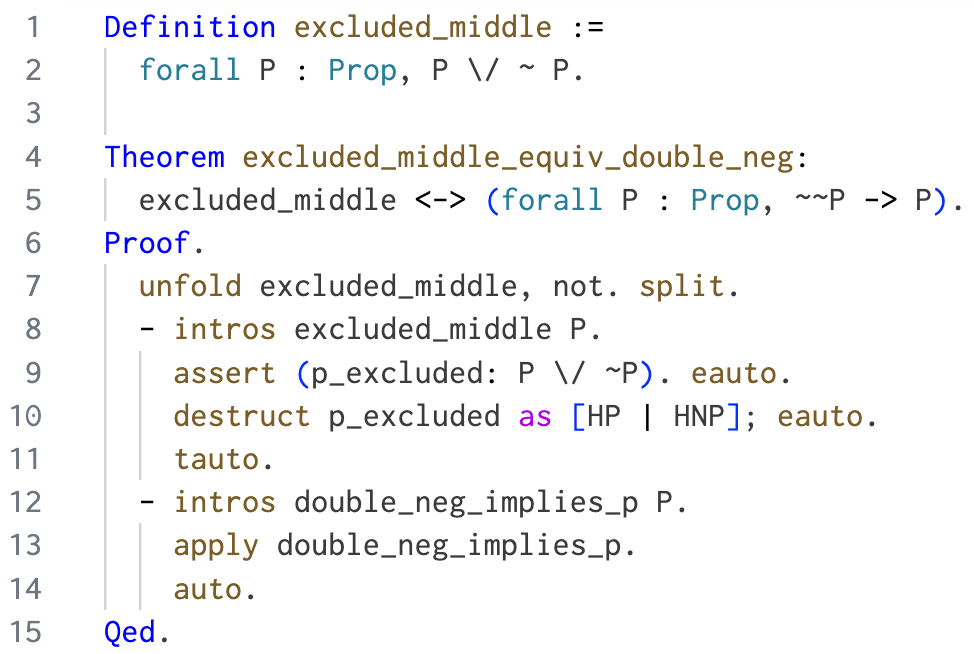
\includegraphics[height=0.95\textheight]{coq-example.png}
    \end{center}
\end{frame}

\section{Coq Usages}

\begin{frame}
    \frametitle{Formalizing Mathematics}

    \begin{itemize}
        \item \textbf{Curry-Howard Correspondence}
        \item \href{https://madiot.fr/coq100/}{\underline{Formalizing 100 theorems in Coq}}
        \begin{itemize}
            \item 4-color Theorem
            \item Irrationality of \(\sqrt{2}\)
            \item Mean Value Theorem
            \item ... and much more!
        \end{itemize}
    \end{itemize}
\end{frame}

\begin{frame}
    \frametitle{Software Verification}

    \begin{itemize}
        \item \textbf{Modeling and verifying software behavior}
        \item \href{https://github.com/coq/coq/wiki/List of Coq PL Projects}{\underline{List of Coq PL Projects}}
        \item CompCert: Optimizing C compiler proven correct
    \end{itemize}
\end{frame}

\section{Examples}
\subsection{Basic Tactics}
\subsection{Program Verification}
\subsection{Elementary Group Theory}
\begin{frame}
    \frametitle{Examples}

    Source code uploaded at \href{https://github.com/calofmijuck/presentations/tree/main/intro-coq}{\underline{Github}}

    \vspace*{10px}

    \begin{itemize}
        \setlength{\itemsep}{2em}
        \item Basic Tactics
        \item Program Verification
        \item Elementary Group Theory
    \end{itemize}
\end{frame}


\frame{\titlepage}

% \begin{frame}
%   \frametitle{References}
%   \bibliographystyle{unsrt}
%   \linespread{1.1}
%   {\tiny \bibliography{reference.bib}}
% \end{frame}

\end{document}
